\documentclass{template/openetcs_article}
% Use the option "nocc" if the document is not licensed under Creative Commons
%\documentclass[nocc]{template/openetcs_article}
\usepackage{rotating,color}
\usepackage{lipsum,url}
\graphicspath{{./template/}{.}{./images/}}
\begin{document}
\frontmatter
\project{openETCS}

%Please do not change anything above this line
%============================
% The document metadata is defined below

%assign a report number here
\reportnum{OETCS/WP7/T7.1}

%define your workpackage here
\wp{Work-Package 7: ``Benchmark''}

%set a title here
\title{Classical B models}

%set a subtitle here
\subtitle{Introduction and notes on classical B models}

%set the date of the report here
\date{May 2013}

%define a list of authors and their affiliation here

\author{Marielle Petit-Doche}
\affiliation{Systerel}


% define the coverart
\coverart[width=350pt]{openETCS_EUPL}
 
%define the type of report
\reporttype{Notes}


\begin{abstract}
This document gives a description of the models developed in Classical B  during the benchmark task T7.1.

\end{abstract}

%=============================
%Do not change the next three lines
\maketitle
\tableofcontents
\listoffiguresandtables
\newpage
%=============================


\begin{tabular}{|p{4.4cm}|p{8.7cm}|}
\hline
\multicolumn{2}{|c|}{Document information} \\
\hline
Work Package &  WP7  \\
Deliverable ID or doc. ref. & \\
\hline
Document title & Classical B models \\
Document version & 00.01 \\
Document authors (org.)  & Marielle Petit-Doche (Systerel) \\
\hline
\end{tabular}

\begin{tabular}{|p{4.4cm}|p{8.7cm}|}
\hline
\multicolumn{2}{|c|}{Review information} \\
\hline
Last version reviewed &  \\
\hline
Main reviewers &  \\

\hline
\end{tabular}

\begin{tabular}{|p{2.2cm}|p{4cm}|p{4cm}|p{2cm}|}
\hline
\multicolumn{4}{|c|}{Approbation} \\
\hline
  &  Name & Role & Date   \\
\hline  
Written by    &  Marielle Petit-Doche &  & \\
\hline
Approved by &  &  & \\
\hline
\end{tabular}

\begin{tabular}{|p{2.2cm}|p{2cm}|p{3cm}|p{5cm}|}
\hline
\multicolumn{4}{|c|}{Document evolution} \\
Version &  Date & Author(s) & Justification  \\
\hline
00.01 & 25/05/2013 & M. Petit-Doche &  Document creation  \\
\hline  
\end{tabular}

% The actual document starts below this line
%=============================


%%%%%%%%%%%%%%%%%%%%%%%%%%%%%%%%%%%%%%%%%%%%%%%%%%%%%%%%%%%%%%
%%%              My macros (=> Sylvain Baro)               %%%
%%%%%%%%%%%%%%%%%%%%%%%%%%%%%%%%%%%%%%%%%%%%%%%%%%%%%%%%%%%%%%
\newcommand{\tbd}{\colorbox{cyan}{\%\%To Be Defined\%\%}}
\newcommand{\tbc}{\colorbox{cyan}{\%\%To Be Confirmed\%\%}}
\newcommand{\todo}[1]{\colorbox{cyan}{\%\%{#1}\%\%}}
\newlength{\origindent}

\newenvironment{issue}{
        \begin{quote}
        \begin{itshape}Open Issue.
}{
        \end{itshape}
        \end{quote}
}

\newenvironment{comment}{
        \begin{quote}
        \begin{itshape}Comment.
}{
        \end{itshape}
        \end{quote}
}

\newenvironment{justif}{
        \begin{quote}
        \begin{itshape}Justification.
}{
        \end{itshape}
        \end{quote}
}


%------------------------------------------
% DEFINITION DES CARACTERES MATHEMATIQUES B
%------------------------------------------
\def\@setmcodes#1#2#3{{\count0=#1 \count1=#3
	\loop \global\mathcode\count0=\count1 \ifnum \count0<#2
	\advance\count0 by1 \advance\count1 by1 \repeat}}

\@setmcodes{`A}{`Z}{"7441}
\@setmcodes{`a}{`z}{"7461}

\mathcode`\;="8000 % Makes ; active in math mode
{\catcode`\;=\active \gdef;{\semicolon\;}}
\mathchardef\semicolon="003B
%    Nominal distance from top of paper to top of page
\topmargin 0 pt
\textheight 53\baselineskip

%   Left margin on odd-numbered pages
\oddsidemargin  0.15 in
%   Left margin on even-numbered pages
\evensidemargin 0.35 in
%   Width of marginal notes.
\marginparwidth 1 in
%   Note that \oddsidemargin = \evensidemargin
\oddsidemargin 0.25 in
\evensidemargin 0.25 in
\marginparwidth 0.75 in
\textwidth 5.875 in % Width of text line.

\setlength{\parindent}{0pt}
\setlength{\parskip}{0ex}

% DEFINITION DES FONTS
%---------------------
% The AMS extra symbol fonts are loaded.
% Note: sometimes called euxm10
\font\msx=msam10
% Note: sometimes called euym10
\font\msy=msbm10

\newfam\msxfam \textfont\msxfam=\msx
\newfam\msyfam \textfont\msyfam=\msy

\def\famletter#1{\ifcase #1 0\or 1\or 2\or 3\or 4\or 5\or 6\or 7\or
	8\or 9\or A\or B\or C\or D\or E\or F\fi}

\edef\fx{\famletter\msxfam}
\edef\fy{\famletter\msyfam}

\def\bbold{\fam\msyfam \msy}

% SYMBOLES B
%-----------
% makes a quoted expression in mathematical text
\def\token#1{\hbox{`$#1$'}}
% used for error messages in Z specs
\def\report#1{\hbox{`{\tt #1}'}}

% \@myop makes an operator, with a strut to defeat TeX's vertical adjustment.
\def\@myop#1{\mathop{\mathstrut{#1}}\nolimits}

% This underscore doesn't have the little kern --- you get an italic
% correction anyway in math mode.
\def\_{\leavevmode \vbox{\hrule width0.5em}}

% Save \q as \xq for quantifiers q.
\let\xforall=\forall
\let\xexists=\exists
\let\xlambda=\lambda
\let\xmu=\mu

% \p and \f make arrows with 1 and 2 crossings resp.
\def\p#1{\mathrel{\ooalign{\hfil$\mapstochar\mkern 5mu$\hfil\cr$#1$}}}
\def\f#1{\mathrel{\ooalign{\hfil
	$\mapstochar\mkern 3mu\mapstochar\mkern 5mu$\hfil\cr$#1$}}}

\let\mc=\mathchardef

\def	\pow		{\mbox{${\cal P}$}}
\def	\po1		{\mbox{${\cal P}_1$}}
\let	\cross		\times
\def	\lambda		{\@myop{\xlambda}}
\def	\lnot		{\neg\;}
\def	\land		{\mathrel{\wedge}}
\def	\lor		{\mathrel{\vee}}
\let	\implies	\Rightarrow
\let	\iff		\Leftrightarrow
\def	\forall		{\@myop{\xforall}}
\def	\exists		{\@myop{\xexists}}
\def	\semi		{\mathrel{\comp}}
\def	\ssemi		{\mathbin{\rm ;}}
\let	\ensembleVide	\emptyset
\let	\rel		\leftrightarrow
\def	\dom		{\@myop{\sf dom}}
\def	\ran		{\@myop{\sf ran}}
\def	\id		{\@myop{\sf id}}
\def	\comp		{\mathbin{\raise
			0.6ex\hbox{\oalign{\hfil$\scriptscriptstyle
			\rm o$\hfil\cr\hfil$\scriptscriptstyle\rm 9$\hfil}}}}
\def	\para		{\mbox{$\mid\mid$}}
\mc	\dres		"2\fx43
\mc	\rres		"2\fx42
\def	\ndres		{\mathbin{{\dres} \llap{$-$}}}
\def	\nrres		{\mathbin{{\rres}\llap{$-$}}}
\def	\lover		{\mathbin{{\dres} \llap{$-\!\!\!\!-\!$}}}
\def	\rover		{\mathbin{{\rres}\llap{$\!-\!\!\!-$}}}
\let	\fun		\rightarrow
\def	\pfun		{\p\fun}
\def	\pinj		{\p\inj}
\mc	\inj		"3\fx1A
\def	\psurj		{\p\surj}
\mc	\surj		"3\fx10
\def	\bij		{\surj\!\!\!\!\!\!\!\inj}
\def	\nat		{\mbox{${\cal N}$}}
\def	\na1		{\mbox{${\cal N}_1$}}
\def	\num		{\mbox{${\cal Z}$}}
\def	\int		{\mbox{${\cal Z}$}}
\def	\rat		{\mbox{${\cal Q}$}}
\def	\div		{\mathbin{\rm /}}
\def	\mod		{\mathbin{\bf mod}}
\def	\upto		{\mathbin{\ldotp\ldotp}}
\def	\finset		{\mbox{${\cal F}$}}
\def	\finse1		{\mbox{${\cal F}_1$}}
\def	\ffun		{\f\fun}
\def	\finj		{\f\inj}
\def	\seq		{\@myop{\rm seq}}
\def	\cat		{\mathbin{\raise 0.8ex\hbox{$\mathchar"2\fx61$}}}
\def	\sep		{\hspace*{.05in}}



\newpage
%------------------------------------------

% Start here


\section{Introduction}
% Start here

\subsection{Classical B method}
The B-Method is a formal method developed by J-R. Abrial and used in industry, especially in railway industry, to develop complex systems. It covers software development from formal specifications to code level. Proof mechanisms guaranty the consistency of specifications properties and the complete consistency of code regarding its formal specification. It is efficient to model  functional  elements of a critical software with respect to  EN50128 constraints.

Classical B has been used successfully  in railway  industry (mainly by Alstom, Siemens and AREVA) to  develop critical software in urban (CBTC, PMI,...) and mainline domains (KVB, Eurobalise,...). Hundred of different systems are running in the world embedding software developed in B (see \url{http://www.cs.vu.nl/~wanf/pubs/handbookFFM.pdf}, \url{http://link.springer.com/chapter/10.1007/3-540-48119-2_22} and \url{http://web.tiscali.it/chiccoterri/Metod B.htm}).


Classical B  is well adapted to describe how a system works and to develop functional  critical software. It can be completed with the Event B method to cover system analyses and to explain why a system works.

The main publication on the method is :

[Abrial1996] The B Book, Assigning Programs to Meanings


Language is documented with language manual reference of the tool Atelier B (\url{http://www.atelierb.eu/ressources/manrefb1.8.6.uk.pdf}). Industrial have developed their own coding rules and guidelines.



\subsection{Atelier B toolkit}

AtelierB is the industrial  tool the most used to develop critical software following the Classical approach.
The tool is partly open-source, but it is free for use.
For more details \url{http://www.atelierb.eu/outil-atelier-b/}.


Tool is documented with the user manual (\url{http://www.tools.clearsy.com/resources/User_uk.pdf}). 

The version of the tool used to develop the models in the sequel is 4.0.2.
However the models can be read on a more recent version of the tool.

\subsection{Benchmark activities}

The rest of the document describes the models developed in Classical B during the benchmark activities of WP7. The examples specified are those proposed as high priority in D2.5.

\begin{description}
\item[State machines] procedure On-sight: § 5.9 of subset 026
\item[Time-outs] Establishing a communication session: §3.5.3 of subset 026
\item[Arithmetic] Braking curves: parts of § 3.13 of subset 026
\item[Truth tables and logical statements] Transition tables: parts of § 4.6.2 and § 4.6.3 of subset 026 
\end{description}


\section{Software Architecture of the model}
% Start here

\subsection{Introduction}

The first step when developing a Classical B  model is to define the architecture of the software to model.

The language allows to give a structure to the model close to the one of the software implemented.
Thus functions are shared between components : those in charge of scheduling the functions, those in charge of managing the inputs, those in charge of managing the output, those in charge of describing the functions in details...  This allows a modular development of the software.

In Classical B, to describe a function (or a set of functions) we need at least two components :  an abstract machine which gives an abstract specification of the functions, and an implementation to detail the functions as an implementable code (by convention the implementation has the same name as the abstract machine with the suffix "\_i"). As much refinement components as necessary can be added between an abstract machine and an implementation to refine step by step the abstract specification until the implementation and to facilitate traceability. Refinement components are usually used only in the case of complex functions. This is the first mean to structure a Classical B model with abstraction level (this can be compared with the distinction between spec and body components of language such as C, Ada or Java).

The second means to structure the Classical B  models is to link the group of components together. Then in a given machine or implementation :
\begin{description}
\item[the SEES clause] allows to link the components which can be viewed in the component : Variables can be read but not modified (it works as "with" clause in C, Ada or Java software)
\item[the IMPORT clause] allows to link the components whom variables can be modified with call of functions (it works as "use" clause in C, Ada or Java software).
\end{description}


\subsection{ETCS  case study}


Figure \ref{fig:graphe} gives the architecture of the ETCS example developed during benchmark activities. Arrows show IMPORT relations.

 \begin{figure}
  \centering
  \fbox{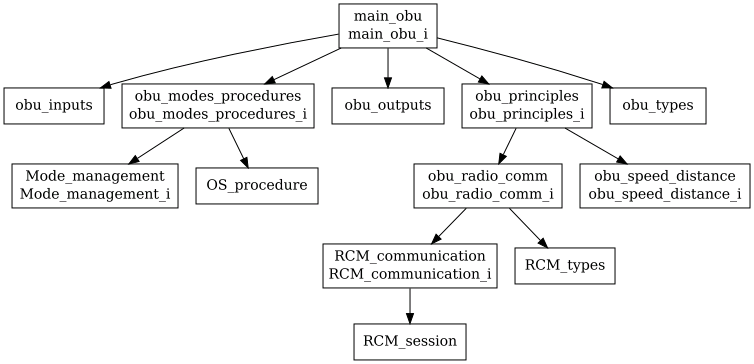
\includegraphics[scale=0.75]{graphe.png}}
  \caption{Classical B  model architecture}
  \label{fig:graphe}
\end{figure}


\begin{description}
\item[main\_obu] is the main sequencer of the software
\item[obu\_types] contains the definition of types and constants used by all the software components. This machine is seen by all the other components.
\item[obu\_inputs] stores the input values in different variables. This machine is seen by most of the other components.
\item[obu\_outputs] manages the outputs.
\item[obu\_modes\_procedures] and branches below are in charge of the management of modes and procedures (subset 26 chapter 4 and 5).
\item[obu\_principles] and branches below are in charge of the functions (chapter 3 of subset 26).
\end{description}

\subsubsection{Main sequencer}

This is the main sequencer with two operation called by the hardware. We assume an applicative cycle is defined and at each cycle the main operation "cycle" is called. The operation "power\_up" is called when the system is started.

\fbox{
\begin{minipage}{14cm}

\bf MACHINE

\hspace*{0.20in}\it main\_obu

\hspace*{0.20in}

\hspace*{0.20in}\bf OPERATIONS

\hspace*{0.20in}

\hspace*{0.20in}\bf power\_up \rm =

\hspace*{0.20in}\bf BEGIN

\hspace*{0.40in}\bf skip

\hspace*{0.20in}\bf END \rm ;

\hspace*{0.20in}

\hspace*{0.20in}\bf cycle \rm =

\hspace*{0.20in}\bf BEGIN

\hspace*{0.40in}\bf skip

\hspace*{0.20in}\bf END

\vspace*{12mm}
\bf END
\end{minipage}
}

\vspace*{8mm}

The implementation gives the sequence of the main operations called at each cycle and during the initialisation. first the inputs at read (we assume here the inputs are read  and stored at the beginning of each cycle and not on the fly). The called operation are defined in the imported components.


\fbox{
\begin{minipage}{14cm}


\bf IMPLEMENTATION

\hspace*{0.15in}\it main\_obu\_i

\bf REFINES

\hspace*{0.20in}\it main\_obu

\vspace*{4mm}
\bf IMPORTS

\hspace*{0.20in}\it obu\_inputs\rm ,

\hspace*{0.20in}\it obu\_modes\_procedures\rm ,

\hspace*{0.20in}\it obu\_principles\rm ,

\hspace*{0.20in}\it obu\_outputs\rm , 

\hspace*{0.20in}\it obu\_types

\vspace*{4mm}
\bf OPERATIONS

\hspace*{0.15in}\bf power\_up \rm =

\hspace*{0.15in}\bf BEGIN

\hspace*{0.35in}\bf initial\_read\_inputs \rm ;

\hspace*{0.35in}\bf intialize\_mode \rm ; \hspace*{0.35in}

\hspace*{0.35in}\bf initialize\_data \rm ; \hspace*{0.35in}

\hspace*{0.35in}\bf initial\_send\_outputs

\hspace*{0.15in}\bf END

\hspace*{0.15in}\rm ;

\vspace*{4mm}
\hspace*{0.15in}\bf cycle \rm =

\hspace*{0.15in}\bf VAR \it vv \bf IN

\hspace*{0.35in}\bf read\_inputs \rm ;

\hspace*{0.35in}\it vv  $\leftarrow$  \bf get\_V\_train \rm ;

\hspace*{0.35in}\bf modes\_procedures\_management\rm (\it vv\rm ) \rm ; \hspace*{0.75in}

\hspace*{0.35in}\bf principles\_management \rm ; \hspace*{0.20in}

\hspace*{0.35in}\bf send\_outputs

\hspace*{0.15in}\bf END

\vspace*{8mm}
\bf END

\end{minipage}
}


\vspace*{8mm}

\subsubsection{Types}

The component obu\_types  defines the types and constants used by the whole system as modes, level,..

\fbox{
\begin{minipage}{14cm}


\bf MACHINE

\hspace*{0.20in}\it obu\_types

\hspace*{0.20in}

\bf SETS

\it t\_mode \rm = \rm \{\it FS\rm , \it LS\rm , \it OS\rm , \it SR\rm , \it SH\rm , \it UN\rm , \it PS\rm , \it SL\rm , \it SB\rm , \it TR\rm , \it PT\rm , \it SF\rm , \it ISo\rm , \it NP\rm , \it NL\rm , \it SN\rm , \it RV\rm \}

\rm ;

\it t\_mamode \rm = \rm \{\it ma\_OS\rm , \it ma\_SH\rm , \it ma\_LS\rm , \it ma\_unknown\rm \}

\rm ;

\it t\_level \rm = \rm \{\it level\_0\rm , \it level\_1\rm , \it level\_2\rm , \it level\_3\rm , \it level\_NTC\rm \}

\rm ;

\it t\_procedure \rm = \rm \{\it NoProcedure\rm , \it StartOfMission\rm , \it EndOfMission\rm , \it SHInitiatedByDriver\rm ,

 \it SHOrderFromTrackside\rm , \it Override\rm , \it OnSight\rm , \it LevelTransitions\rm , \it TrainTrip\rm , 
 
 \it ChangeTrainOrientation\rm , \it TrainReversing\rm , \it Joining\rm , \it Splitting\rm , \it RBCHandover\rm , 
 
\it LevelCrossing\rm , \it ChangingTrainData\rm , \it TrackConditions\rm , \it LimitedSupervision\rm \}

\vspace*{4mm}
\bf CONSTANTS

\hspace*{0.20in}\it VITESSE

\hspace*{0.20in}

\bf PROPERTIES

\hspace*{0.20in}\it VITESSE  $\subseteq$  \bf NAT  $\land$ 

\hspace*{0.20in}\it VITESSE \rm = \rm 0 $\upto$ \rm 6\rm 0\rm 0

\vspace*{4mm}
\bf END

\end{minipage}
}

\newpage





\section{Procedure On-sight (§5.9)}
% Start here

\fbox{
\begin{minipage}{14cm}

\end{minipage}
}


\vspace*{8mm}


\fbox{
\begin{minipage}{14cm}

\end{minipage}
}


\vspace*{8mm}




\section{Communication session (§3.5.3)}
% Start here

\fbox{
\begin{minipage}{14cm}

\end{minipage}
}


\vspace*{8mm}


\fbox{
\begin{minipage}{14cm}

\end{minipage}
}


\vspace*{8mm}




\section{Bracking Curves (§3.13)}
% Start here

\fbox{
\begin{minipage}{14cm}

\end{minipage}
}


\vspace*{8mm}


\fbox{
\begin{minipage}{14cm}

\end{minipage}
}


\vspace*{8mm}



\section{Transition table (§4.6.2)}
% Start here

this section is fully implemented in Classical B in the component Mode\_management and Mode\_management\_i

\fbox{
\begin{minipage}{14cm}


\bf MACHINE

\hspace*{0.20in}\it Mode\_management

\bf SEES

\hspace*{0.20in}\it obu\_types\rm ,

\hspace*{0.20in}\it obu\_inputs

\bf DEFINITIONS

\hspace*{0.20in}\it condition\_1 \rm == \rm (\it driver\_isolate \rm =\hspace*{0.10in}\bf TRUE\rm ) \rm ;

\hspace*{0.20in}\it condition\_5\rm (\it v\_train\rm , \it ll\rm ) \rm == \rm ( \it v\_train \rm = \rm 0  $\land$  \it ll  $\in$  \rm \{\it level\_0\rm , \it level\_NTC\rm , \it level\_1\rm \}  

\hspace*{0.40in} $\land$  \it driver\_ask\_SH \rm = \bf TRUE\rm ) \rm ;

\hspace*{0.20in}\it condition\_6\rm (\it v\_train\rm , \it ll\rm ) \rm == \rm ( \it v\_train \rm = \rm 0\hspace*{0.10in} $\land$  \it ll  $\in$  \rm \{\it level\_2\rm , \it level\_3\rm \} 

\hspace*{0.40in} $\land$  \it driver\_ask\_SH \rm =\hspace*{0.10in}\bf TRUE\rm ) \rm ;

\hspace*{0.20in}\it condition\_10 \rm == \rm ( \it Valid\_Train\_Data \rm =\hspace*{0.10in}\bf TRUE  $\land$  \it Valid\_MA \rm =\hspace*{0.10in}\bf TRUE  

\hspace*{0.40in} $\land$  \it Valid\_SSP \rm =\hspace*{0.10in}\bf TRUE  $\land$  \it Valid\_Grad \rm =\hspace*{0.10in}\bf TRUE  $\land$  \it M\_MAMODE \rm =\hspace*{0.10in}\it ma\_unknown\rm ) \rm ;

\hspace*{0.20in}\it condition\_50 \rm == \rm (\it SH\_request\_accepted \rm =\hspace*{0.10in}\bf TRUE  $\land$  \it driver\_ack \rm =\hspace*{0.10in}\bf TRUE\rm )


\bf OPERATIONS

\hspace*{0.20in}\it mm\rm , \it ll\rm , \it pr  $\leftarrow$  \it manage\_mode\rm (\it pm\rm , \it pl\rm , \it vv\rm , \it ppr\rm ) \rm =

\hspace*{0.20in}\bf PRE

\hspace*{0.40in}\it pm  $\in$ \hspace*{0.10in}\it t\_mode  $\land$ 

\hspace*{0.40in}\it pl  $\in$ \hspace*{0.10in}\it t\_level  $\land$ 

\hspace*{0.40in}\it vv  $\in$ \hspace*{0.10in}\it VITESSE  $\land$ 

\hspace*{0.40in}\it mm  $\in$  \it t\_mode  $\land$ 

\hspace*{0.40in}\it ll  $\in$  \it t\_level  $\land$ 

\hspace*{0.40in}\it pr  $\in$  \it t\_procedure  $\land$ 

\hspace*{0.40in}\it ppr  $\in$  \it t\_procedure  $\land$ 

\hspace*{0.40in} $\neg$  \rm ( \rm (\it condition\_5\rm (\it vv\rm , \it pl\rm )  $\lor$  \it condition\_6\rm (\it vv\rm , \it pl\rm )\rm )  $\land$  \it condition\_50 \rm )  $\land$ 

\hspace*{0.40in} $\neg$ \rm ( \rm (\it condition\_5\rm (\it vv\rm , \it pl\rm )  $\lor$  \it condition\_6\rm (\it vv\rm , \it pl\rm )\rm )  $\land$  \it condition\_10\hspace*{0.10in}\rm )  $\land$ 

\hspace*{0.40in} $\neg$ \rm ( \it condition\_50  $\land$  \it condition\_10\hspace*{0.10in}\rm )
\hspace*{0.20in}\bf THEN

\hspace*{0.40in}\it mm\rm , \it ll\rm , \it pr\hspace*{0.10in}\rm :\rm (

\hspace*{0.60in}\it mm  $\in$  \it t\_mode  $\land$ 

\hspace*{0.60in}\it ll  $\in$  \it t\_level  $\land$ 

\hspace*{0.60in}\it pr  $\in$  \it t\_procedure  $\land$ 

\hspace*{0.60in}\rm ( \it condition\_1\hspace*{0.10in} $\implies$  \rm ( \it mm \rm = \it ISo  $\land$  \it ll \rm = \it pl  $\land$  \it pr \rm = \it ppr\rm ) \rm )  $\land$ 

\hspace*{0.60in}\rm (  $\neg$ \rm (\it condition\_1\rm )  $\implies$  \rm (

\hspace*{0.80in}\rm ( \rm ( \it condition\_5\rm (\it vv\rm , \it pl\rm )  $\lor$  \it condition\_6\rm (\it vv\rm , \it pl\rm ) \rm )\hspace*{0.25in}

\hspace*{1.00in} $\land$  \it pm \rm = \it SB  $\implies$  \rm ( \it mm \rm = \it SH  $\land$  \it ll \rm = \it pl  $\land$  \it pr \rm = \it ppr\rm ) \rm )  $\land$ 

\hspace*{0.80in}\rm ( \it condition\_50 

\hspace*{1.00in} $\land$  \it pm \rm = \it SB  $\implies$  \rm ( \it mm \rm = \it SH\hspace*{0.10in} $\land$  \it ll \rm = \it pl  $\land$  \it pr \rm = \it SHInitiatedByDriver\rm ) \rm )  $\land$ 

\hspace*{0.80in}\rm ( \it condition\_10 

\hspace*{1.00in} $\land$  \it pm \rm = \it SB  $\implies$  \rm ( \it mm \rm = \it FS  $\land$  \it ll \rm = \it pl  $\land$  \it pr \rm = \it ppr\rm ) \rm )  $\land$ 

\hspace*{0.80in}\rm (  $\neg$ \rm (\it condition\_5\rm (\it vv\rm , \it pl\rm )  $\lor$  \it condition\_6\rm (\it vv\rm , \it pl\rm )  $\lor$  \it condition\_50  $\lor$  \it condition\_10\rm ) 

\hspace*{1.00in} $\land$  \it pm \rm = \it SB  $\implies$  \rm ( \it mm \rm = \it pm  $\land$  \it ll \rm = \it pl  $\land$  \it pr \rm = \it ppr\rm ) \rm )  $\land$ 

\hspace*{0.80in}\rm ( $\neg$ \rm (\it pm\rm =\it SB\rm )  $\implies$  \rm ( \it mm \rm = \it pm  $\land$  \it ll \rm = \it pl  $\land$  \it pr \rm = \it ppr\rm ) \rm )

\hspace*{0.80in}\rm ) \rm )  $\land$ 

\hspace*{0.60in}\rm ( \it pm \rm = \it ISo  $\implies$  \it mm \rm = \it ISo \rm )\hspace*{0.25in} $\land$ 

\hspace*{0.60in}\rm ( \rm (\it driver\_isolate \rm = \bf FALSE  $\land$  \it pm  $\not =$  \it ISo\rm )  $\implies$ \hspace*{0.10in}\it mm  $\not =$  \it ISo \rm )\hspace*{0.40in}

\hspace*{0.60in}\rm )

\hspace*{0.20in}\bf END

\bf END

\end{minipage}
}


\newpage


\fbox{
\begin{minipage}{14cm}


\bf IMPLEMENTATION

\hspace*{0.15in}\it Mode\_management\_i

\bf REFINES

\hspace*{0.15in}\it Mode\_management

\bf SEES

\hspace*{0.15in}\it obu\_types \rm ,

\hspace*{0.15in}\it obu\_inputs

\bf OPERATIONS

\hspace*{0.15in}\it mm \rm , \it ll \rm , \it pr  $\leftarrow$  \it manage\_mode \rm ( \it pm \rm , \it pl \rm , \it vv \rm , \it ppr\rm ) \rm =

\hspace*{0.15in}\bf VAR \it di\rm , \it daSH\rm , \it SHra\rm , \it da\rm , \it vtd\rm , \it vma\rm , \it vssp\rm , \it vg\rm , \it mma \bf IN

\hspace*{0.35in}\it mm \rm := \it pm \rm ;

\hspace*{0.35in}\it ll \rm := \it pl \rm ;

\hspace*{0.35in}\it pr \rm := \it ppr \rm ;

\hspace*{0.35in}\it di  $\leftarrow$  \bf get\_driver\_isolate \rm ;

\hspace*{0.35in}\bf IF \it di \rm = \bf TRUE\hspace*{0.10in}\hspace*{0.35in}\bf

\hspace*{0.35in} THEN

\hspace*{0.55in}\it mm \rm := \it ISo\hspace*{0.10in}\hspace*{0.35in}\bf

\hspace*{0.35in} ELSE

\hspace*{0.55in}\bf IF \it pm \rm = \it SB\hspace*{0.10in}

\hspace*{0.55in}\bf  THEN

\hspace*{0.75in}\it daSH\hspace*{0.10in} $\leftarrow$  \bf get\_driver\_ask\_SH\rm ;

\hspace*{0.75in}\bf IF \rm (\it vv \rm = \rm 0  $\land$  \it daSH \rm = \bf TRUE\rm )

\hspace*{0.75in}\bf THEN

\hspace*{0.95in}\it mm \rm := \it SH

\hspace*{0.75in}\bf ELSE

\hspace*{0.95in}\it da\hspace*{0.10in} $\leftarrow$  \bf get\_driver\_ack \rm ;

\hspace*{0.95in}\it SHra\hspace*{0.10in} $\leftarrow$  \bf get\_SH\_request\_accepted\rm ;

\hspace*{0.95in}\bf IF \rm (\it da \rm =\hspace*{0.10in}\bf TRUE  $\land$  \it SHra \rm = \bf TRUE \rm ) 

\hspace*{0.95in}\bf  THEN

\hspace*{1.15in}\it mm \rm :=\hspace*{0.10in}\it SH \rm ;

\hspace*{1.15in}\it pr \rm := \it SHInitiatedByDriver 

\hspace*{0.95in}\bf ELSE\hspace*{0.15in}

\hspace*{1.20in}\it vtd  $\leftarrow$  \bf get\_Valid\_Train\_Data \rm ;

\hspace*{1.20in}\it vma  $\leftarrow$  \bf get\_Valid\_MA \rm ;

\hspace*{1.20in}\it vssp  $\leftarrow$  \bf get\_Valid\_SSP \rm ;

\hspace*{1.20in}\it vg  $\leftarrow$  \bf get\_Valid\_Grad \rm ;

\hspace*{1.20in}\it mma  $\leftarrow$  \bf get\_M\_MAMODE \rm ;

\hspace*{1.20in}\bf IF \it vtd \rm =\hspace*{0.10in}\bf TRUE  $\land$  \it vma \rm = \bf TRUE  $\land$  \it vssp \rm = \bf TRUE  $\land$ 

\hspace*{1.40in} \it vg \rm = \bf TRUE  $\land$  \it mma \rm = \it ma\_unknown

\hspace*{1.20in}\bf  THEN

\hspace*{1.40in}\it mm \rm := \it FS 

\hspace*{1.20in}\bf  ELSE

\hspace*{1.40in}\bf skip

\hspace*{1.20in}\bf END

\hspace*{1.00in}\bf END

\hspace*{0.80in}\bf END

\hspace*{0.60in}\bf END

\hspace*{0.40in}\bf END

\hspace*{0.20in}\bf END

\vspace*{8mm}
\bf END

\end{minipage}
}


\newpage

The property \textbf{PROPERTY\_4.6.2\_01}  "OBU shall never enter in isolated mode if not requested by the driver", is specified as postcondition of the operation of obu\_modes\_procedures :

\fbox{
\begin{minipage}{14cm}

( \rm (\it driver\_isolate \rm = \bf FALSE  $\land$  \it previous\_mode  $\not =$  \it ISo\rm )  $\implies$ \hspace*{0.10in}\it M\_mode  $\not =$  \it ISo \rm )
	
\end{minipage}
}
	    
	    \vspace*{8mm}
		    
The property \textbf{PROPERTY\_4.6.2\_02}   "OBU shall never leave Isolated mode (no transition from Isolation is specified) ie. if system  was previously  isolate, it stay isolate", is specified as an invariant of obu\_modes\_procedures :

\fbox{
\begin{minipage}{14cm}

\rm ( \it previous\_mode \rm = \it ISo  $\implies$  \it M\_mode \rm = \it ISo \rm )


\end{minipage}
}







%%%%%%%%%%%%%%%%%%%%%%%%%%%

%% Bibliography
\nocite{*}
\bibliographystyle{unsrt}
\bibliography{erdc}
\bibliography{process}



% \begin{thebibliography}{9}

% \bibitem{lamport94}
  % Leslie Lamport,
  % \emph{\LaTeX: A Document Preparation System}.
  % Addison Wesley, Massachusetts,
  % 2nd Edition,
  % 1994.

% \end{thebibliography}

%===================================================
%Do NOT change anything below this line

\end{document}
